
%(BEGIN_QUESTION)
% Copyright 2006, Tony R. Kuphaldt, released under the Creative Commons Attribution License (v 1.0)
% This means you may do almost anything with this work of mine, so long as you give me proper credit

The {\it integral} function appears in a variety of physical systems encountered in process measurement and control applications.  One such application is liquid flow.  Shown here is a liquid-holding vessel equipped with a vortex flow indicator for measuring incoming liquid flow and a level indicator for measuring liquid volume accumulating in the vessel:

$$\includegraphics[width=15.5cm]{i01578x01.eps}$$

If you were to graph both the liquid flow rate ($Q$) and the liquid volume ($V$) accumulated in the vessel over time, which of these two variables would be the {\it integral} of the other with respect to time?  How would you write this in mathematical form, as a calculus expression?

\underbar{file i01578}
%(END_QUESTION)





%(BEGIN_ANSWER)

Volume is the time-integral of flow rate, in this system:

$$V = \int Q \> dt$$

%(END_ANSWER)





%(BEGIN_NOTES)

It should be mentioned to your students that real devices called {\it integrators} exist to take a flowmeter reading and convert it into a total volume measurement.

%INDEX% Mathematics, calculus: integral (accumulated volume as the integral of flow)

%(END_NOTES)


